\chapter{Geokokapen APIa}

Geokokapen APIak erabiltzailearen kokapen zehatza aurkitzeko metodoak eskaintzen ditu. API hau bereziki interesgarria da HTML5 euskarria ematen duten gailu mugikorretan erabiltzeko. W3C erakundeak argitaratutako espezifikazioa bada ere, berez geokokapen APIa ez dago HTML5en espezifikazioaren barruan.
API honen bidez, munduko puntu baten geokokapena lortu ahalko dugu, adibidez: Bilbo, latitudea: 43° 15' iparra, longitudea: 2° 55' mendebaldea.
Ikus dezagun API honen erabileraren adibide bat. Gure helburua uneko geokokapena lortzea izango da.

\begin{figure}[ht]
	\centering
\begin{tikzpicture}
\node[anchor=south west,inner sep=0] (image) at (0,0)
   {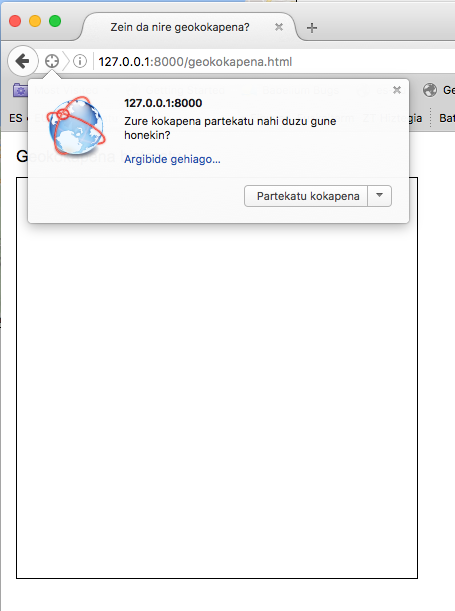
\includegraphics[trim=0cm 0cm 0cm 0cm, clip=true, width=0.5\textwidth]{img/geopermission}};
\end{tikzpicture}
\caption{Geokokapena lortzeko nabigatzaileak erabiltzaileari baimena eskatu behar dio (lehendabiziko aldia bada).}
\label{fig:kokapenabaimena}
\end{figure}

\begin{figure}[ht]
	\centering
\begin{tikzpicture}
\node[anchor=south west,inner sep=0] (image) at (0,0)
   {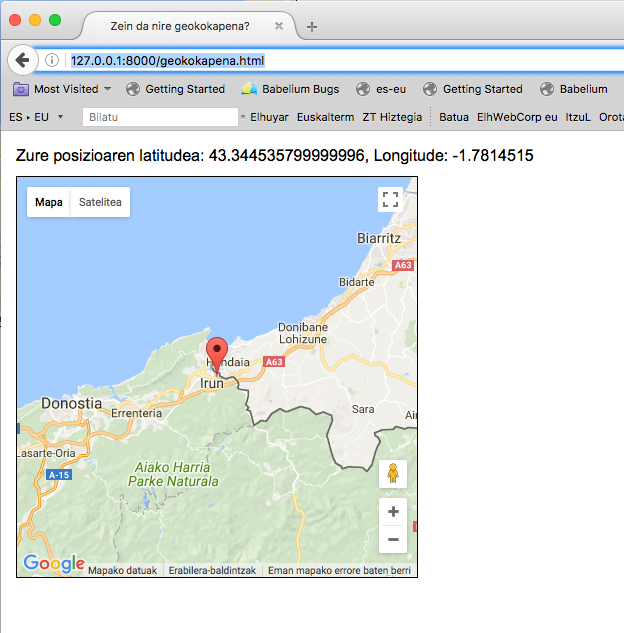
\includegraphics[trim=0cm 0cm 0cm 0cm, clip=true, width=0.5\textwidth]{img/geoapi}};
\end{tikzpicture}
\caption{Google Maps API eta geokokapen APIa erabiliz, uneko kokapena lortu eta mapa batean margotu dugu.}
\label{fig:kokapenagooglemaps}
\end{figure}

\begin{alertinfo}{HTTPS protokoloa erabili geokokapena partekatu ahal izateko}
       Segurtasuna dela eta, ezin da file:// protokoloa erabili geokokapena lortzeko. Alegia, HTTP zerbitzari bat beharko duzu gai honen inguruko ariketak egiteko. Askotan ikasleek file:// protokoloa erabiltzen dute beren probak egiteko. Orain arte horrela egiteak ez zuen inolako oztoporik sortzen, baina orain bai, ordea. Ez baduzu Apache (HTTP zerbitzari ezagunena) instalatu edo konfiguratu nahi, Python erabil dezakezu, modu errazean HTTP zerbitzari bat martxan jarri ahal izateko:

       \$ python -mSimpleHTTPServer 

Komando horrek Pythonek eskaintzen duen HTTP zerbitzari sinple bat martxan jarriko du, 8000 portuan entzunez, uneko karpetaren fitxategiak eskainiz. Orain, nabigatzailean, http://localhost:8000 edo http://127.0.0.1:8000 idatziz, HTTP protokoloa erabili ahalko duzu gai honen ariketak modu erraz batean probatu ahal izateko. Pribatutasuna dela eta, HTTPS da erabili beharreko protokoloa localhost domeinua ez badugu erabiltzen.
\end{alertinfo}

\section{Posizioa lortzen. getCurrentPosition metodoa}

\textit{getCurrentPosition()} \index{getCurrentPosition()} metodoaren sinadura hau da:

\begin{lstlisting}[numbers=none]
getCurrentPosition(callback, errorea, aukerak)   
\end{lstlisting}


Funtzio horri deitzean, nabigatzaileak egiaztatu beharko du ea erabiltzaileak posizioa ezagutzeko baimena eman duen edo ez. Baiezkoan, \textit{callback} funtzioari deituko dio. Ezezkoan, erabiltzaileari galdetu eta haren erantzunaren arabera \textit{callback} edo errore-funtzioari deituko dio (ikus \ref{fig:geolocationapi}. irudia). \textit{Aukerak} izeneko hautazko parametroaren bidez kokapenaren zehaztasun batzuk ezar daitezke.

\begin{lstlisting}[numbers=none,language=JavaScript]
// defektuzko balioak 
let aukerak = {
enableHighAccuracy: false, // zehaztasun maila altua nahi den edo ez
timeout: Infinity,  // asko jota zenbat denbora itxaron behar den geokokapena lortzen errorerik eman gabe
maximumAge: 0 // cachean dauden geokokapenen denbora maximoa berrerabiliak ahal izateko, milisegundutan. 0 = ez erabili cachea
}
\end{lstlisting}

Ikus dezagun adibide zehatz bat (inplementazioa \href{https://codesandbox.io/s/geokokapena-v9vbz?file=/index.html}{hemen\footnote{https://github.com/yuchenlin/rebiber}} proba dezakezu).

\begin{figure}[ht]
	\centering
\begin{tikzpicture}
\node[anchor=south west,inner sep=0] (image) at (0,0)
   {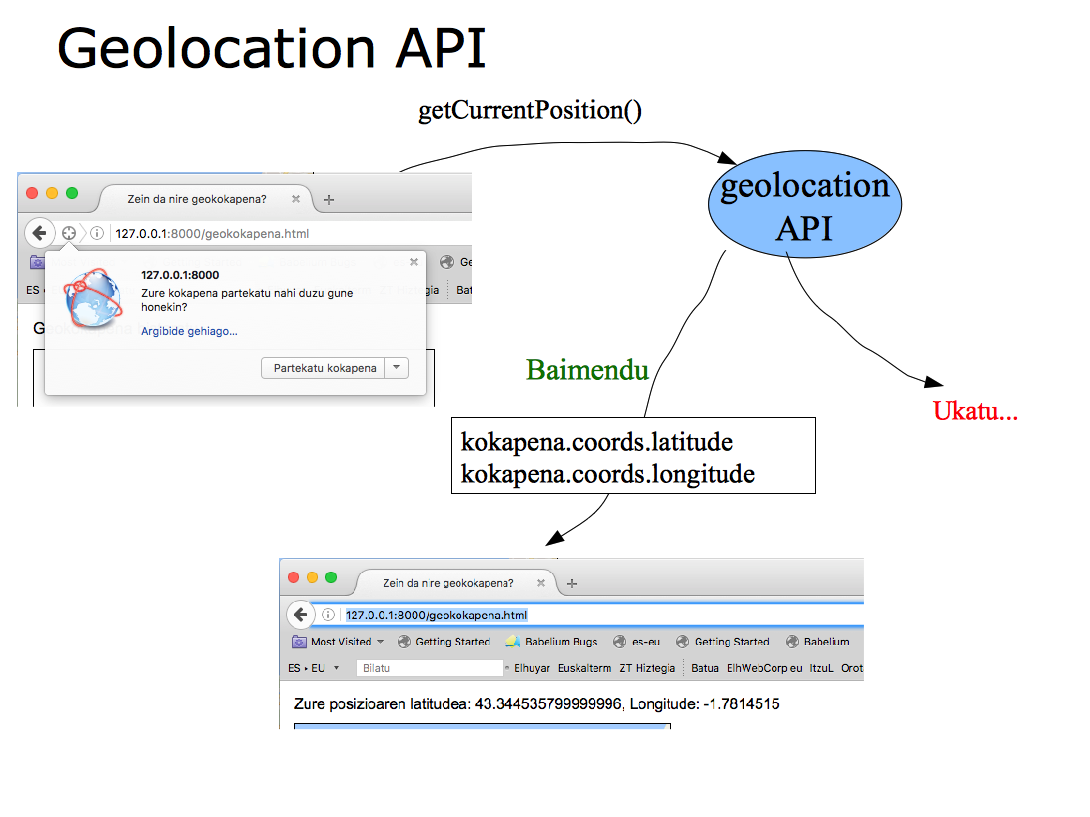
\includegraphics[trim=0cm 0cm 0cm 0cm, clip=true, width=0.5\textwidth]{img/geolocation_api_eu}};
\end{tikzpicture}
\caption{Kokapena: Nola funtzionatzen duen Geolocation \index{Geolocation API} APIak.}
\label{fig:geolocationapi}
\end{figure}

\begin{lstlisting}[language=JavaScript]
window.onload = lortuGeokokapena;

function lortuGeokokapena() {

// nabigatzaileak geolocation APIa inplementatzen du?
	if (navigator.geolocation) {

		navigator.geolocation.getCurrentPosition( bistaratuGeokokapena , bistaratuErrorea);
	}
	else {
		alert("Nabigatzaile honek ez du geokokapen APIa onartzen");
	}
}

function bistaratuGeokokapena(posizioa) {
	let latitude = posizioa.coords.latitude;
	let longitude = posizioa.coords.longitude;

	let div = document.getElementById("geokokapena");
	div.innerHTML = "Zure posizioaren latitudea: " + latitude + ", Longitude: " + longitude;

//	mapaBistaratu(posizioa.coords);

}

function bistaratuErrorea(error) {
	const errorTypes = {
		0: "Errore ezezagun",
		1: "Ez duzu kokapena lortzeko baimenik",
		2: "Kokapena ez dago eskuragarri",
		3: "Itxaron denbora agortu da"
	};
	let errorMessage = errorTypes[error.code];
	if (error.code == 0 || error.code == 2) {
		errorMessage = errorMessage + " " + error.message;
	}
	let div = document.getElementById("geokokapena");
	div.innerHTML = errorMessage;
}
\end{lstlisting}

\begin{alertinfo}{macOS sistema erabiltzen duzu?}
Adi! macOS sistema eragilean bazaude Security\&Privacy fitxan Chrome edo Firefox nabigatzaileei geokokapena lortzeko baimena eman beharko diezu Geolocation APIa erabili ahal izateko.
\end{alertinfo}

\section{Geokokapena Google Maps-en marrazten}
Aurreko kodean erabiltzailearen geokokapena lortu dugu, baina ez dugu mapa batean marraztu. Horretarako, Google Maps-eko APIaren laguntza beharko dugu. Ohart zaitez aurreko kodean 22. lerroa komentatuta dagoela (\textit{mapaBistaratu} metodoari deia). Lerro hori deskomentatu eta jarraian dugun \textit{mapaBistaratu} metodoa aztertu. 

\begin{lstlisting}[language=HTML5]
<head>
<script type="text/javascript" src="//maps.googleapis.com/maps/api/js?key=GAKOA"> </script>
</head>
<body>
<div id="kokapena">
Zure geokokapena hemen bistaratuko da.
</div>
<div id="mapa">
</div>

</body>
</html>
\end{lstlisting}

\begin{alertinfo}{Google Maps API key}
Adi! Google Maps-eko APIa erabiltzeko API gako bat eskatu beharko duzu hemen \href{https://developers.google.com/maps/documentation/javascript/get-api-key}{https://developers.google.com/maps/documentation/javascript/get-api-key}
\end{alertinfo}


\begin{lstlisting}[language=JavaScript]
let map; // aldagai globala

function mapaBistaratu(coords) {
let googleLatAndLong = new google.maps.LatLng(coords.latitude,coords.longitude);

const mapOptions = {
zoom: 10,
center: googleLatAndLong,
mapTypeId: google.maps.MapTypeId.ROADMAP
};

let mapDiv = document.getElementById("mapa");
map = new google.maps.Map(mapDiv, mapOptions);
}
\end{lstlisting}

Bi metodo erabiltzen ari gara hemen, 
\index{google.maps.LatLng}\textit{google.maps.LatLng} (mapan kokatu nahi dugun puntuaren latitudea eta longitudea parametro gisa espero dituena)  eta \textit{google.maps.Map}\index{google.maps.Map} eraikitzailea. Horrek bi parametro jasotzen ditu: \textit{div} etiketa baten erreferentzia (mapa zer geruzatan marraztu nahi dugun jakiteko) eta aukera-objektu bat, \textit{mapOptions}, zer motatako mapa eta zer zoomekin ikusi nahi dugun zehazteko.

Orain arte landutako adibidea \href{https://ikasten.io/html5/geokokapena.html}{https://ikasten.io/html5/geokokapena.html} webgunean aurki dezakezu.

\subsection{Markatzaileak}
Falta zaigun gauza bakarra markatzaile gorri bat jartzea da (\textit{marker} bat). Markatzaile horren gainean klik egitean, gure uneko kokapena agertuko da maparen gainean. Presta dezagun \hl{markatzaileaGehitu} izeneko funtzio bat. 

\begin{lstlisting}[language=JavaScript]
function markatzaileaGehitu(mapa, latlong, izenburua, edukia){
    let markerOptions = {
        position: latlong,
        map: mapa,
        title: izenburua,
        clickable: true
    };
    let marker = new google.maps.Marker(markerOptions);
    

    let infoWindowOptions = {
        content: edukia,
        position: latlong
    };
    let infoWindow = new google.maps.InfoWindow(infoWindowOptions);
    google.maps.event.addListener(marker, "click", function() {
        infoWindow.open(mapa);
    });
}
\end{lstlisting}

Orain \textit{mapaBistaratu()} funtziotik, \textit{markatzaileaGehitu} funtzioari deituko diogu:
\begin{lstlisting}[language=JavaScript]
let izenburua = "Zure kokapena";
let edukia = "Hemen zaude kokatua: " + coords.latitude + ", " + coords.longitude;
markatzaileaGehitu(map, googleLatAndLong, izenburua, edukia);
\end{lstlisting}

Markatzaileak erabiltzen dituen kodearen adibidea online ikusteko, jo ezazu honako helbide honetara: \newline
\href{https://ikasten.io/html5/markadorea.html}{https://ikasten.io/html5/markadorea.html}
\begin{figure}[ht]
	\centering
\begin{tikzpicture}
\node[anchor=south west,inner sep=0] (image) at (0,0)
   {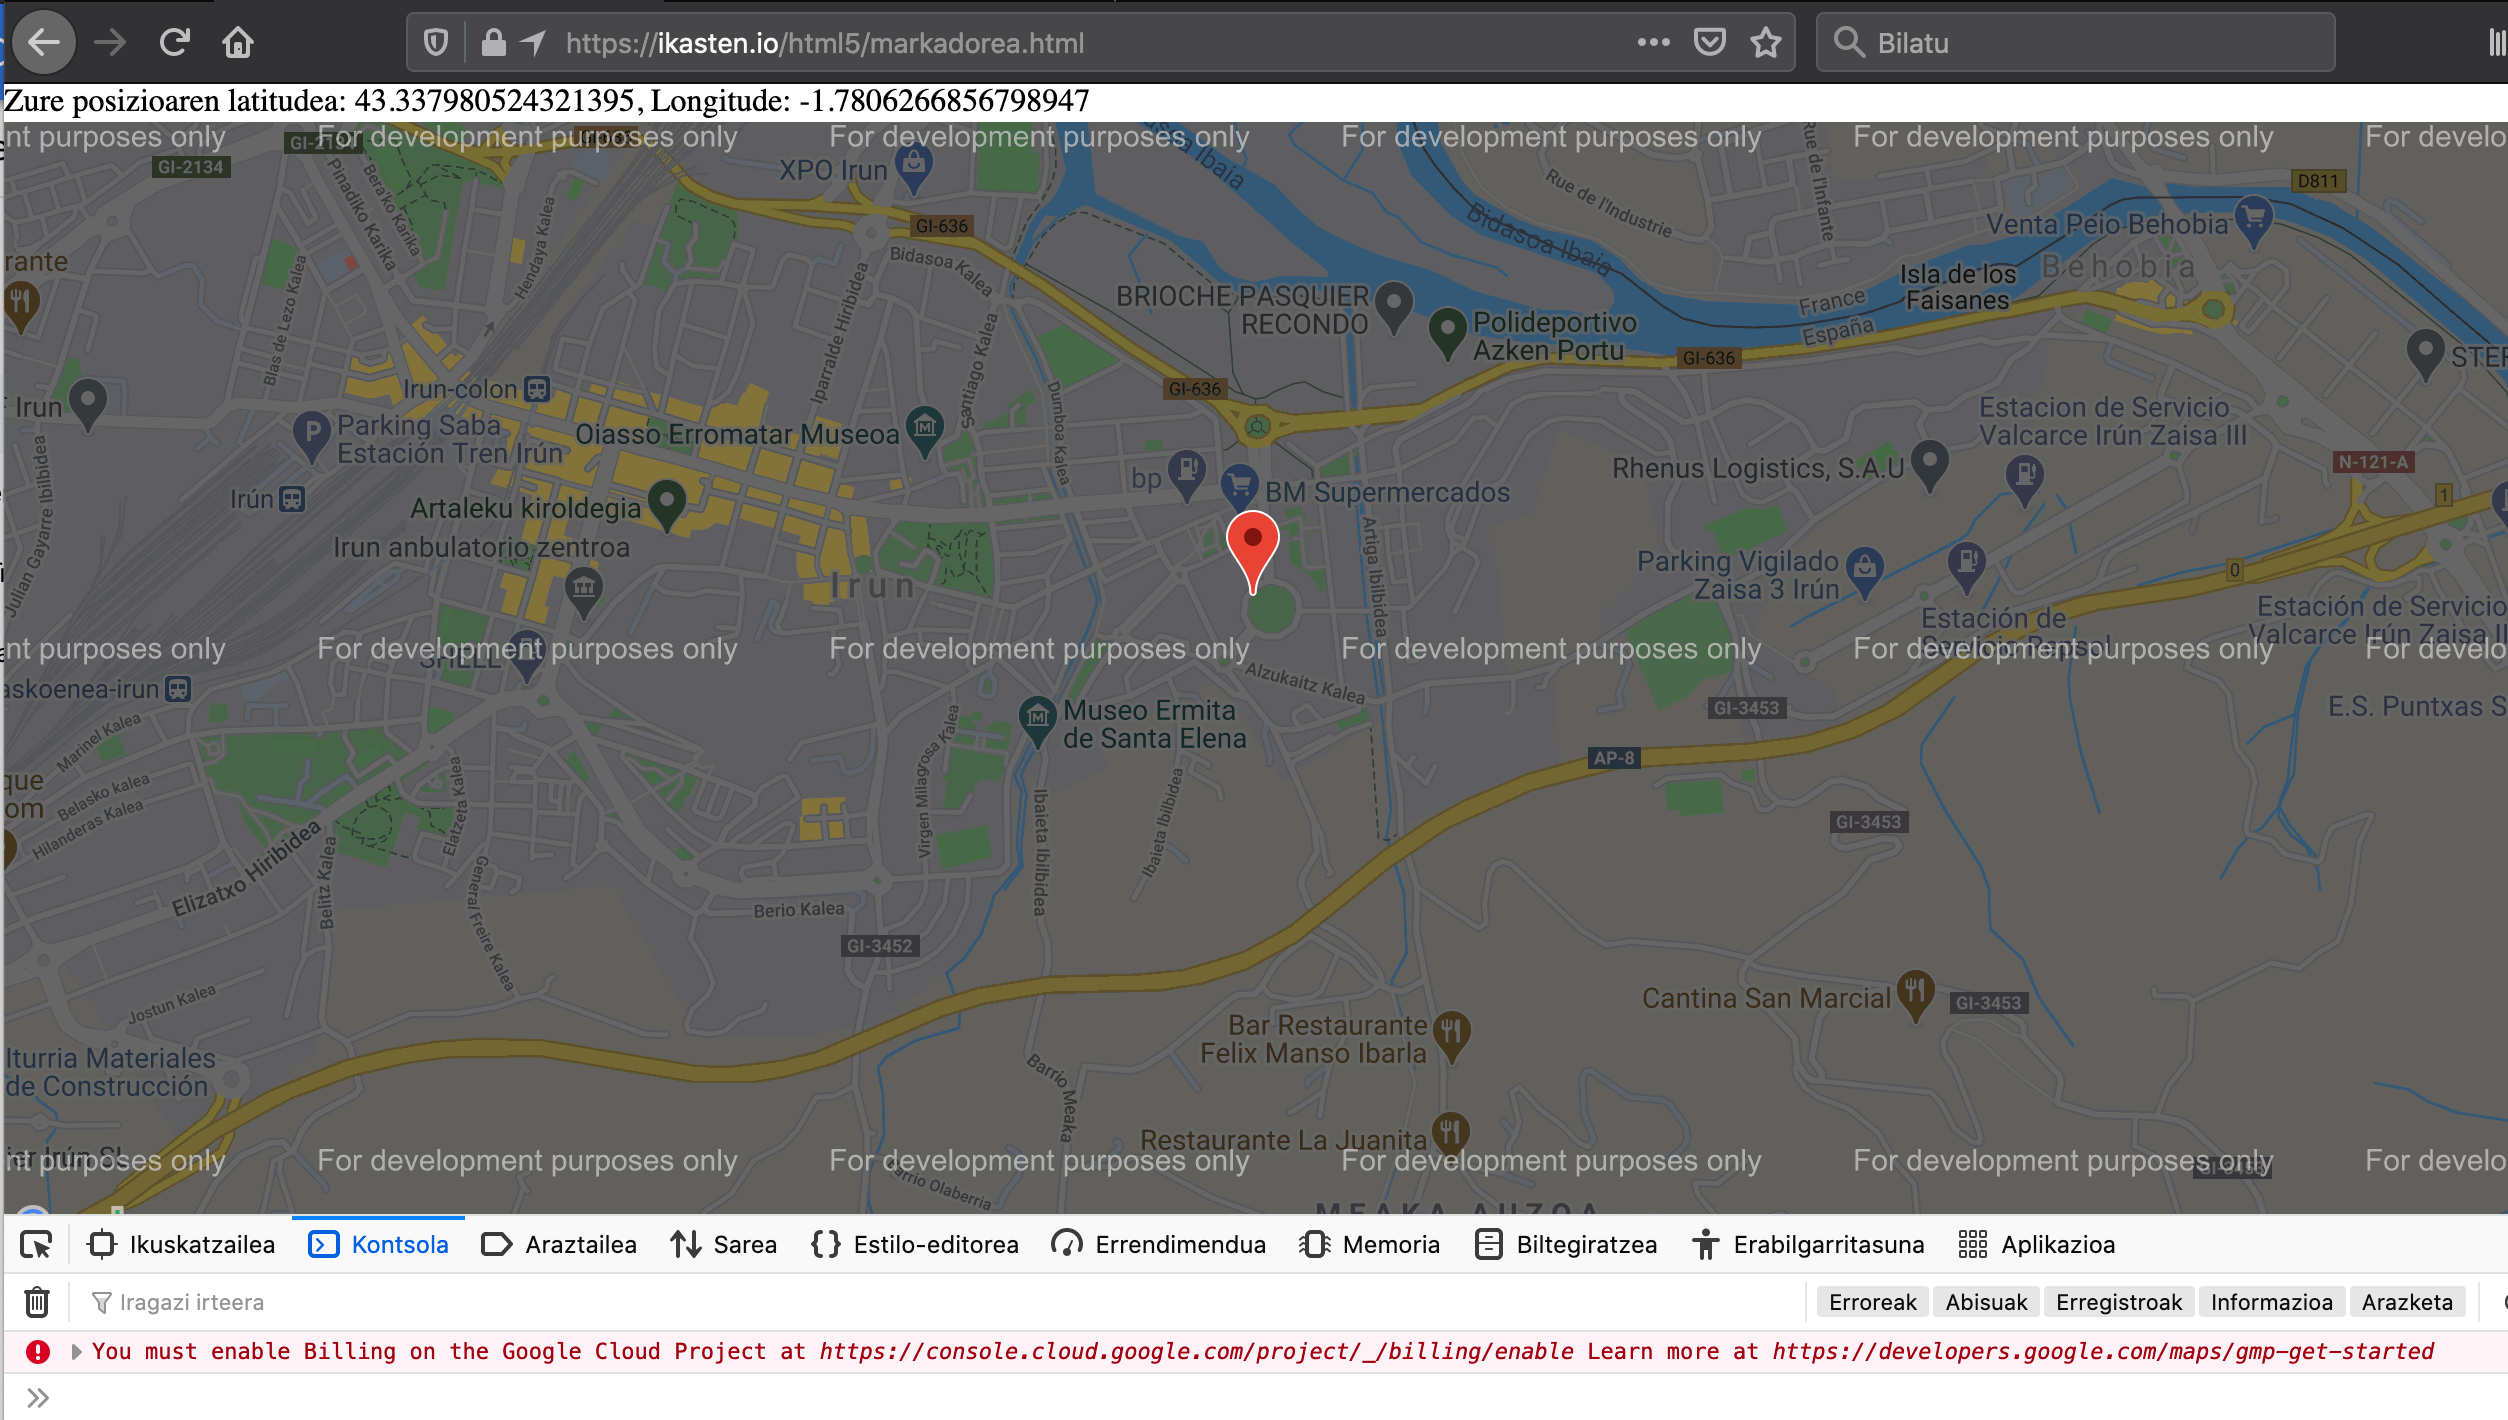
\includegraphics[trim=0cm 0cm 0cm 0cm, clip=true, width=0.75\textwidth]{img/geokokapena/markadorea.png}};
\end{tikzpicture}
\caption{Markatzaileak (mapan agertzen den ikur gorria) Google Maps APIa erabiliz maparen gainean jar daitezke. Ohart zaitez \textit{``For development purposes only''} mezuan eta kontsolan agertzen den mezu gorrian. Mezu horiek kentzeko (eta mapa hobeto ikusteko) ordainpeko kontu bat ireki beharko dugu Google Maps-en honako helbide honetan: \href{https://console.cloud.google.com/project/\_/billing/enable }{https://console.cloud.google.com/project/\_/billing/enable }.}
\label{fig:markadorea}
\end{figure}

\section{Ariketak}

Mugitu ahala zure geokokapena mapa baten gainean bistaratu nahi dugu. Zure geokokapenaren gainean dagoen markatzailean sakatzean, irekitzen den informazio-panelean longitudea eta latitudea bistaratzeaz gain, zauden tokiaren altitudea ere ikusi nahi dugu. Horretarako, Google Maps-ek eskaintzen duen \textit{locationService} APIaren bidez altitudea lortzea eskatzen da. 


Geokokapen APIaren \textit{Coordinates} klaseak hautazko lau parametro eskaintzen ditu (ez daude nabigatzaile guztietan inplementatuta edo ezin dira denak erabili gailu guztietan):
\textit{altitude}, \textit{altitudeAccuracy}, \textit{heading} eta \textit{speed}.

Txantiloi honetan oinarriturik:
\href{https://jsfiddle.net/juanan/jsexk3rh/12/}{https://jsfiddle.net/juanan/jsexk3rh/12/} bertan dagoen JavaScript kodea aldatu markagailu batean klikatzean pantailan uneko posizioa  eta altitudea bistaratu ahal izateko (ikus \ref{fig:maps-ariketa}. irudia). Altueraren datu hori zuzenean eskuratzea posible ez balitz, Google Maps-ek eskaintzen duen elevationService()\footnote{
\textit{elevationService()} metodoaren dokumentazioa hemen aurkituko duzu:\\
\href{https://developers.google.com/maps/documentation/javascript/examples/elevation-simple}{https://developers.google.com/maps/documentation/javascript/examples/elevation-simple}
} zerbitzuari deitu eta hortik eskuratu ahalko duzu\footnote{elevationService() zerbitzutik jasotzen duzun altuera zenbaki erreal gisa bistaratu, bi dezimalera biribilduz (\textit{parseFloat()}\index{parseFloat()} metodoa lagungarria egingo zaizu)}.

\textit{e1elevationService()}\index{elevationService()} metodoa Google Maps-eko 3. bertsiotik aurrera dago eskuragarri. Bertsio
hori nola kargatzen den ikasteko, metodoaren dokumentazioan eskaintzen den adibidearen HTML kodea aztertzea gomendagarria da.


\begin{figure}[ht]
	\centering
\begin{tikzpicture}
\node[anchor=south west,inner sep=0] (image) at (0,0)
   {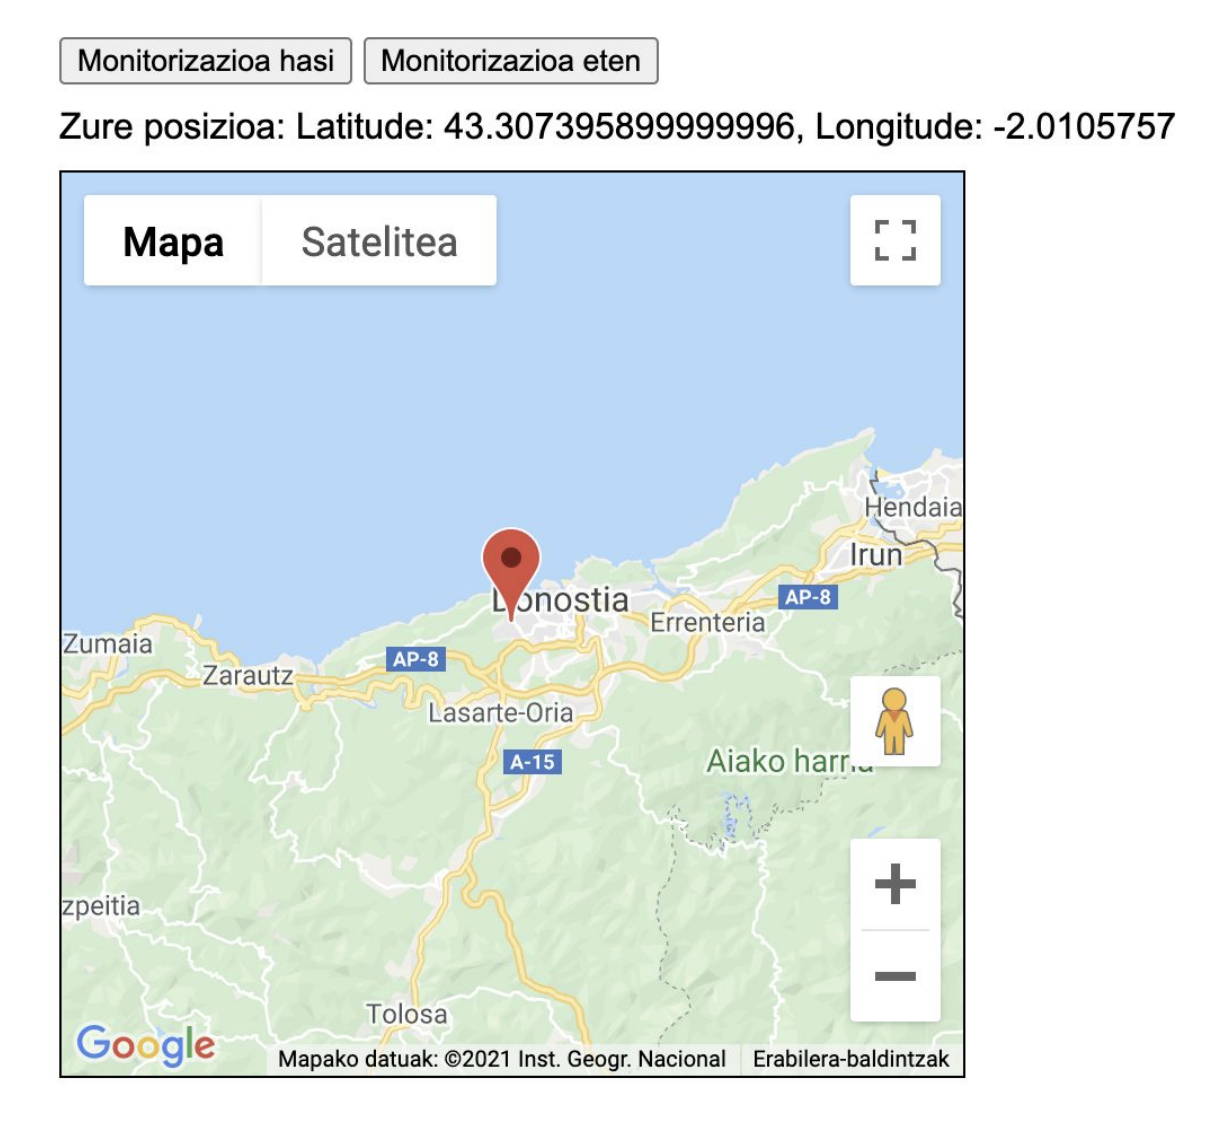
\includegraphics[trim=0cm 0cm 0cm 0cm, clip=true, width=0.5\textwidth]{img/geokokapena/maps-ariketa.png}};
\end{tikzpicture}
\caption{Google Maps-ekin egindako ariketaren emaitza.}
\label{fig:maps-ariketa}
\end{figure}


% \begin{table}[]
% \centering
% \caption{Geokokapen APIak eskaintzen dituen parametro guztiek ez dute derrigorrez balio bat emango. Taulan hautazko eta derrigorrezko atributuak zehazten dira.}
% \label{tab:my-table}
% \begin{tabular}{|l|l|}
% \hline
% \textbf{Coordinates klasea} & \textbf{Geokokapen APIa} \\ \hline
% \begin{tabular}[c]{@{}l@{}}latitude\\ longitude\\ accuracy\end{tabular} & \begin{tabular}[c]{@{}l@{}}Ezker aldeko 3 atributu horiek\\ derrigorrezkoak dira (balio bat itzuli behar\\ dute)\end{tabular} \\ \hline
% \begin{tabular}[c]{@{}l@{}}altitude\\ altitudeAccuracy\\ heading\\ speed\end{tabular} & \begin{tabular}[c]{@{}l@{}}Ezker aldeko 4 atributu horiek hautazkoak\\ dira (batzuetan ez dute baliorik izango)\end{tabular} \\ \hline
% \end{tabular}
% \end{table}
